
\begin{figure*}[ht!]
  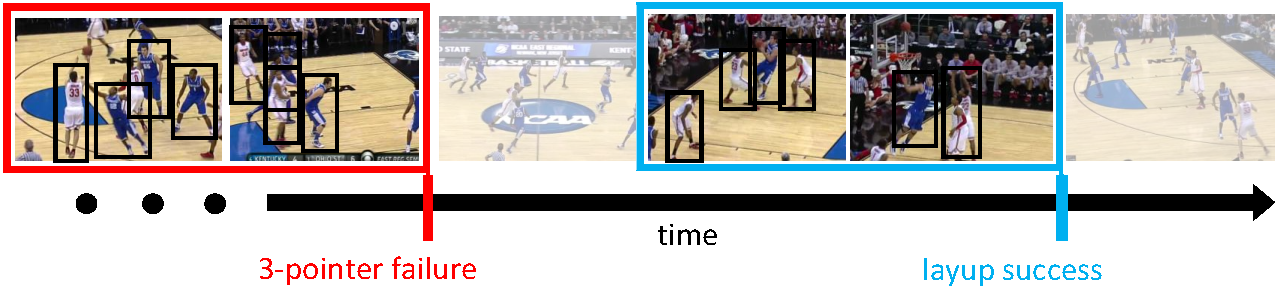
\includegraphics[width=6.5 in]{images/dataset_figure_cropped.pdf}
  \caption{We densely annotate every instance of 11 different basketball events in long basketball
  video. As shown here, we collected the event time-stamp along with the event label through an
AMT task.}
\end{figure*}



\section{Related Work}

\noindent \textbf{Action recognition in videos}
Traditionally, well engineered features have proved quite effective for video
classification and retrieval tasks
\cite{Dalal_ECCV06,Jain_CVPR13,Jiang_ECCV12,Laptev_CVPR08,
Niebels_ECCV10,Oh_MVA14,Oneata_ICCV13,Peng_ECCV14,Sadanand_CVPR12,Schuldt_ICPR04,Wang_BMVC09,Wang_CVPR11}.
The improved dense trajectory (IDT) features \cite{Wang_CVPR11} achieve
competitive results on standard video datasets.  In the last few years,
end-to-end trained deep network models
\cite{Ji_PAMI13,Karpathy_CVPR14,Simonyan_2014,Simonyan_NIPS14,Tran_arxiv14} were shown to be comparable and
at times better than these features for various video tasks.  Other works like
\cite{Wang_arxiv15,Xu_2015,Zha_2015} explore methods for pooling such
features for better performance. Recent works using RNN have achieved
state-of-the-art results for both event recognition and caption-generation
tasks \cite{Donahue_arxiv14,Ng_arxiv15,Srivastava_2015,Yao_arxiv15}.
We follow this line of work with the addition of an attention mechanism
to attend to the event participants.

Another related line of work jointly identifies the region of interest in a video
while recognizing the action.
Gkioxari et al.  \cite{Gkioxari_arxiv14} and Raptis et al.  \cite{Raptis_CVPR12}
automatically localize a spatio-temporal tube in a video.
Jain et al. \cite{Jain_CVPR14} merge super-voxels for action localization.
While these methods perform weakly-supervised action localization, they are targeted
towards single actor videos in short clips.
Other methods like \cite{Lan_ICCV11,Prest_PAMI13,Tian_CVPR13,Wang_ECCV14} require annotations
for the action region or human-joints during training.

%Similarly, Lan et al. \cite{Lan_ICCV11}
%jointly learn a person detector based on image-level anntoations.
\eat{Tian et al. \cite{Tian_CVPR13} train a supervised object detector
while Wang et al. \cite{Wang_ECCV14} train a pose detector with joint annotations
along with the action recognition model.}

%Similarly, \cite{Gkioxari_ICCV15} localize boxes in static images for action recognition.
\noindent \textbf{Muti-person video analysis}
Activity recognition models for events with well defined group structures such
as parades have been presented in
\cite{Vaswani_CVPR03,Intille_CVIU01,Moore_AAAI02,Khan_ACM05}.  They utilize the
structured layout of participants to identify group events. More
recently, \cite{Lan_PAMI12,Choi_ICCV09,Khodabandeh_arxiv15} use context as a
cue for recognizing interaction-based group activities.  While they work with 
multi-person events, these methods are restricted to smaller
datasets such as UT-Interaction\cite{Ryoo_10}, Collective activity
\cite{Choi_ICCV09} and Nursing home\cite{Lan_PAMI12}.

\noindent \textbf{Attention models}
Itti et al. \cite{Itti_PAMI98} explored the idea of saliency-based attention in
images, with other works like \cite{Shapovalova_NIPS13} using eye-gaze data as
a means for learning attention.  Mnih et al. \cite{Mnih_NIPS14} attend to
regions of varying resolutions in an image through a RNN framework.  Along
similar lines, attention has been used for image classification
\cite{Cao_ICCV15,Gregor_arxiv15,Xiao_arxiv14} and detection
\cite{Ba_arxiv14,Caicedo_ICCV15,Yoo_arxiv15} as well.

Bahdanau et al. \cite{Bahdnau_arxiv14} showed that attention-based RNN models
can effectively align input words to output words for machine translation.
Following this, Xu et al. \cite{Xu_arxiv15} and Yao et al. \cite{Yao_arxiv15}
used attention for image-captioning and video-captioning respectively.
\eat{Following this work, attention was used for aligning regions in an image to
output words for image-captioning \cite{Xu_arxiv15} and frames in a video with
output words for video-captioning \cite{Yao_arxiv15}.} In all these methods,
attention aligns a sequence of input features with words of an output sentence.
However, in our work we use attention to identify the most relevant person to
the overall event during different phases of the event.\eat{We also provide a
better BLSTM based representation for the attended people as
discussed in Section~\ref{sec:methods}.}

\noindent \textbf{Action recognition datasets}
Action recognition in videos has evolved with the introduction of more
sophisticated datasets starting from smaller KTH \cite{KTH}, HMDB \cite{HMDB}
to larger , UCF101 \cite{UCF101}, TRECVID-MED \cite{MED11} and Sports-1M
\cite{Karpathy_CVPR14} datasets.  More recently, THUMOS \cite{THUMOS} and
ActivityNet \cite{ActivityNet} also provide a detection setting with temporal
annotations for actions in untrimmed videos.  There are also fine-grained
datasets in specific domains such as MPII cooking \cite{Finegrained_cooking}
and breakfast \cite{Breakfast}.  However, most of these datasets focus on
single-person activities with hardly any need for recognizing the people
responsible for the event. On the other hand, publicly available multi-person
activity datasets like \cite{Ryoo_10,Choi_ICCV09,VIRAT} are restricted to a very small
number of videos.  One of the contributions of our work is a multi-player
basketball dataset with dense temporal event annotations in long videos.

\noindent \textbf{Person detection and tracking}. There is a very
large literature on person detection and tracking. Here we just
mention a few key papers.
For person detection, we use the CNN-based multibox detector from
\cite{Szegedy13}.
For person tracking, we use the KLT tracker from
\cite{Veenman_PAMI2001}.
There is also work on player identification (e.g., \cite{Lu2013}), but
in this work, we do not attempt to distinguish individual players.
